\documentclass{ximera}
\usepackage{OERLinearAlgebra}


\usepackage{mathtools}
\usepackage{tikz-3dplot}
\usetikzlibrary{shapes.geometric}
\usetikzlibrary{arrows}

\author{Anna Davis \and Paul Zachlin} \title{Linear Independence} \license{CC-BY 4.0}

\begin{document}

\begin{abstract}
 We define linear independence and relate it to the concept of redundant vectors.
\end{abstract}
\maketitle


Recall that given a set of vectors $\{\vec{v}_1,\vec{v}_2,\ldots ,\vec{v}_p\}$, an element $\vec{v}_i$ of the set is called \dfn{redundant} if $\vec{v}_i$ can be expressed as a linear combination of the other vectors in the set.  

In VEC-M-0090 we found that a redundant vector can be added to, or removed from the spanning set without affecting the span.  The idea of redundancy generalizes to one of the most fundamental ideas of linear algebra -- linear independence.

%Our goal is to establish a general procedure for determining whether a given set of vectors contains redundant vectors.

%The set  $\{\vec{v}_1,\vec{v}_2,\ldots ,\vec{v}_p\}$ contains a redundant vector if and only if there are scalars $a_1,\ldots ,a_{i-1}, a_{i+1},\ldots ,a_p$ such that 
%$$\vec{v}_i=a_1\vec{v}_1+\ldots +a_{i-1}\vec{v}_{i-1}+a_{i+1}\vec{v}_{i+1}+\ldots +a_p\vec{v}_p$$
%for some $1\leq i\leq p$.
%This equation is satisfied if and only if $(a_1,\ldots ,a_{i-1},-1, a_{i+1},\ldots ,a_p)$
%$$-\vec{v}_i+a_1\vec{v}_1+\ldots +a_{i-1}\vec{v}_{i-1}+a_{i+1}\vec{v}_{i+1}+\ldots +a_p\vec{v}_p=\vec{0}$$

\begin{initprob}\label{init:onlytrivialrelation}
Consider
$$\left\{\begin{bmatrix}3\\-1\\3\end{bmatrix}, \begin{bmatrix}-2\\4\\1\end{bmatrix},\begin{bmatrix}2\\-1\\1\end{bmatrix}\right\}$$
Does this set contain redundant vectors?  Let's form a linear combination of the three vectors:
$$a_1\begin{bmatrix}3\\-1\\3\end{bmatrix}+a_2 \begin{bmatrix}-2\\4\\1\end{bmatrix}+a_3\begin{bmatrix}2\\-1\\1\end{bmatrix}$$
Next, we will form a vector equation by setting this linear combination equal to the zero vector.
\begin{align}\label{eq:onlytrivialrelation1}a_1\begin{bmatrix}3\\-1\\3\end{bmatrix}+a_2 \begin{bmatrix}-2\\4\\1\end{bmatrix}+a_3\begin{bmatrix}2\\-1\\1\end{bmatrix}=\vec{0}\end{align}

Solving this equation for $a_1$, $a_2$ and $a_3$ will allow us to express one of the vectors (say, $\begin{bmatrix}-2\\4\\1\end{bmatrix}$) as a linear combination of the others:
\begin{align}\label{eq:onlytrivialrelation2}\begin{bmatrix}-2\\4\\1\end{bmatrix}=-\frac{a_1}{a_2}\begin{bmatrix}3\\-1\\3\end{bmatrix}-\frac{a_3}{a_2}\begin{bmatrix}2\\-1\\1\end{bmatrix}\end{align}
But there is a catch.  Can you think of a case where the linear combination in (\ref{eq:onlytrivialrelation2}) would be undefined?

If you guessed that $a_2=0$ would cause a problem, you are correct.  But even if $a_2=0$, we may still be able to find a redundant vector by solving (\ref{eq:onlytrivialrelation1}) for a different vector, like so:

$$\begin{bmatrix}3\\-1\\3\end{bmatrix}=-\frac{a_2}{a_1}\begin{bmatrix}-2\\4\\1\end{bmatrix}-\frac{a_3}{a_1}\begin{bmatrix}2\\-1\\1\end{bmatrix}$$
But what if $a_1=0$?

If we find that $a_1=a_2=a_3=0$ is the only solution to
$$a_1\begin{bmatrix}3\\-1\\3\end{bmatrix}+a_2 \begin{bmatrix}-2\\4\\1\end{bmatrix}+a_3\begin{bmatrix}2\\-1\\1\end{bmatrix}=\vec{0}$$ 
we will conclude that none of the three vectors can be written as a linear combination of the others, and therefore there are no redundant vectors in the set.

Converting this vector equation to augmented matrix form and performing row reduction yields

$$\left[\begin{array}{ccc|c}  
 3&-2&2&0\\-1&4&-1&0\\3&1&1&0
 \end{array}\right]\rightsquigarrow\left[\begin{array}{ccc|c}  
 1&0&0&0\\0&1&0&0\\0&0&1&0
 \end{array}\right]$$
 
This means that $a_1=a_2=a_3=0$ is the only solution, and there are no redundant vectors in the set.
\end{initprob}

Exploration Problem \ref{init:onlytrivialrelation} makes a convincing case that one of the three vectors can be expressed as a linear combination of the other two if and only if at least one of $a_1, a_2, a_3$ is not equal to zero.  This observation motivates the following definition.

\begin{definition}[Linear Independence]\label{def:linearindependence}
Let $\vec{v}_1, \vec{v}_2,\ldots ,\vec{v}_p$ be vectors of $\RR^n$.  We say that $\vec{v}_1, \vec{v}_2,\ldots ,\vec{v}_p$ are \dfn{linearly dependent} if there exist scalars $a_1, a_2, \ldots , a_p$, not all zero, such that
\begin{align}\label{eq:defoflinind}a_1\vec{v}_1+a_2\vec{v}_2+\ldots +a_p\vec{v}_p=\vec{0}\end{align}
Otherwise we say that $\vec{v}_1, \vec{v}_2,\ldots ,\vec{v}_p$ are \dfn{linearly independent}.
\end{definition}

The expression in    (\ref{eq:defoflinind}) is called a \dfn{linear relation} among the vectors $\vec{v}_1, \vec{v}_2,\ldots ,\vec{v}_p$.   Clearly, the \dfn{trivial relation} ($a_1=a_2=\ldots =a_p=0$) always exists.  If the trivial relation is the only possible linear relation, then we say that the vectors $\vec{v}_1, \vec{v}_2,\ldots ,\vec{v}_p$ are linearly independent.  If, in addition to the trivial relation, a \dfn{non-trivial relation} (not all $a_1, a_2,\ldots ,a_p$ are zero) exists, then we say that vectors $\vec{v}_1, \vec{v}_2,\ldots ,\vec{v}_p$ are linearly dependent.

\begin{example}\label{ex:linind}Determine whether the vectors in each part are linearly independent.

\begin{enumerate}
\item \label{item:linindpart1}
$$\begin{bmatrix}2\\-3\end{bmatrix}, \begin{bmatrix}0\\3\end{bmatrix},\begin{bmatrix}1\\-1\end{bmatrix},\begin{bmatrix}1\\-2\end{bmatrix}$$

\item \label{item:linindpart2} $$\begin{bmatrix}2\\1\\4\end{bmatrix},\begin{bmatrix}-3\\1\\1\end{bmatrix}$$
\end{enumerate}
\begin{explanation} \ref{item:linindpart1}
We will solve the vector equation
\begin{align}\label{eq:linrelationpart1}a_1\begin{bmatrix}2\\-3\end{bmatrix}+a_2 \begin{bmatrix}0\\3\end{bmatrix}+a_3\begin{bmatrix}1\\-1\end{bmatrix}+a_4\begin{bmatrix}1\\-2\end{bmatrix}=\vec{0}\end{align}
 
 Clearly $a_1=a_2=a_3=a_4=0$ is a solution to the equation.  The question is whether another solution exists.
 
The vector equation translates into the following system:

$$\begin{array}{ccccccccc}
      2a_1 & &&+&a_3&+&a_4&= &0 \\
        -3a_1& +&3a_2&-&a_3&-&2a_4&= &0 \\
      \end{array}$$
  Writing the system in augmented matrix form and applying elementary row operations gives us the following reduced row-echelon form:
  $$\left[\begin{array}{cccc|c}  
 2&0&1&1&0\\-3&3&-1&-2&0
 \end{array}\right]\rightsquigarrow\left[\begin{array}{cccc|c}  
 1&0&1/2&1/2&0\\0&1&1/6&-1/6&0
 \end{array}\right]$$
 This shows that (\ref{eq:linrelationpart1}) has infinitely many solutions:  
 $$a_1=-\frac{1}{2}s-\frac{1}{2}t,\quad a_2=-\frac{1}{6}s+\frac{1}{6}t,\quad a_3=s,\quad a_4=t$$
 Letting $t=s=6$, we obtain the following non-trivial linear relation:
 
 $$-6\begin{bmatrix}2\\-3\end{bmatrix}+0 \begin{bmatrix}0\\3\end{bmatrix}+6\begin{bmatrix}1\\-1\end{bmatrix}+6\begin{bmatrix}1\\-2\end{bmatrix}=\vec{0}$$
 We conclude that the vectors are linearly dependent.
 
 \ref{item:linindpart2} We need to solve the equation
 
 $$a_1\begin{bmatrix}2\\1\\4\end{bmatrix}+a_2\begin{bmatrix}-3\\1\\1\end{bmatrix}=\vec{0}$$
 Converting the equation to augmented matrix form and performing row reduction gives us
 $$\left[\begin{array}{cc|c}  
 2&-3&0\\1&1&0\\4&1&0
 \end{array}\right]\rightsquigarrow\left[\begin{array}{cc|c}  
 1&0&0\\0&1&0\\0&0&0
 \end{array}\right]$$
 This shows that $a_1=a_2=0$ is the only solution.  Therefore the two vectors are linearly independent.
\end{explanation}

\end{example}


\begin{example}\label{ex:linearlydependentindependent}
In Example \ref{ex:redundantvectors} of VEC-M-0090 we introduced two spanning sets:
$$\left\{\begin{bmatrix}5\\0\\4\end{bmatrix}, \begin{bmatrix}0\\4\\2\end{bmatrix},\begin{bmatrix}5\\4\\6\end{bmatrix}\right\}$$
and
$$\left\{\begin{bmatrix}5\\0\\4\end{bmatrix}, \begin{bmatrix}0\\4\\2\end{bmatrix},\begin{bmatrix}4\\5\\0\end{bmatrix}\right\}$$
Recall that we found the vector $\begin{bmatrix}5\\4\\6\end{bmatrix}$ to be redundant of the first two vectors. We also found that the second set contains no redundant vectors. 

\begin{enumerate}
\item\label{item:linearlydependent}
Show that the vectors
$$\begin{bmatrix}5\\0\\4\end{bmatrix}, \begin{bmatrix}0\\4\\2\end{bmatrix},\begin{bmatrix}5\\4\\6\end{bmatrix}$$
are linearly dependent.
\item\label{item:linearlyindependent}
Show that the vectors
$$\begin{bmatrix}5\\0\\4\end{bmatrix}, \begin{bmatrix}0\\4\\2\end{bmatrix},\begin{bmatrix}4\\5\\0\end{bmatrix}$$ are linearly independent.
\end{enumerate}

\begin{explanation}
\ref{item:linearlydependent} Observe that a non-trivial linear relation exists:

$$\begin{bmatrix}5\\0\\4\end{bmatrix}+ \begin{bmatrix}0\\4\\2\end{bmatrix}-\begin{bmatrix}5\\4\\6\end{bmatrix}=\vec{0}$$
We conclude that the three vectors in the spanning set are linearly dependent.

\ref{item:linearlyindependent}
Showing that the three vectors are linearly independent may be hard to do by observation.  We resort to solving the vector equation:

$$a_1\begin{bmatrix}5\\0\\4\end{bmatrix}+ a_2\begin{bmatrix}0\\4\\2\end{bmatrix}+a_3\begin{bmatrix}4\\5\\0\end{bmatrix}=\vec{0}$$

This vector equation translates into the following augmented matrix and reduces to its reduced row-echelon form as follows:

$$\left[\begin{array}{ccc|c}  
 5&0&4&0\\0&4&5&0\\4&2&0&0
 \end{array}\right]\rightsquigarrow\left[\begin{array}{ccc|c}  
 1&0&0&0\\0&1&0&0\\0&0&1&0
 \end{array}\right]$$
 
 We conclude that $a_1=a_2=a_3=0$ is the only solution to the equation.  Thus, the vectors are linearly independent.
\end{explanation}
\end{example}
To formalize the connection between linear dependence and redundant vectors we prove the following theorem.
\begin{theorem}
A set of vectors is linearly dependent if and only if it contains redundant vectors.
\end{theorem}
\begin{proof}
Suppose the set $\{\vec{v}_1,\vec{v}_2,\ldots ,\vec{v}_p\}$ contains a redundant vector $\vec{v}_i$.  Then there exist scalars $a_1, a_2,\ldots, a_{i-1},a_{i+1},\ldots ,a_p$ such that
$$\vec{v}_i=a_1\vec{v}_1+a_2\vec{v}_2+\ldots +a_p\vec{v}_p$$
But then 
$$-\vec{v}_i+a_1\vec{v}_1+a_2\vec{v}_2+\ldots +a_p\vec{v}_p=\vec{0}$$
is a non-trivial relation among the vectors.  Thus $\vec{v}_1,\vec{v}_2,\ldots ,\vec{v}_p$ are linearly dependent.

Conversely, suppose that the vectors $\vec{v}_1,\vec{v}_2,\ldots ,\vec{v}_p$ are linearly dependent.  Then there exist scalars $a_1, a_2, \ldots ,a_p$, not all zero, such that
$$a_1\vec{v}_1+a_2\vec{v}_2+\ldots +a_p\vec{v}_p=\vec{0}$$
Suppose $a_i\neq 0$, then
$$\vec{v}_i=-\frac{a_1}{a_i}\vec{v}_1-\frac{a_2}{a_i}\vec{v}_2-\ldots -\frac{a_p}{a_i}\vec{v}_p$$
Therefore $\vec{v}_i$ is redundant because it can be written as a linear combination of the other vectors.
\end{proof}

%\section*{Introduction to Homogeneous Systems}

%You have probably noticed that determining linear dependence or independence of vectors requires us to solve a linear system in which every constant term is equal to zero.  Such a linear system is called \dfn{homogeneous}.

%A homogeneous system translates into an augmented matrix with zeros to the right of the vertical bar. As we perform elementary row operations, the entries on the right-hand side remain zero.  Knowing this makes it unnecessary to keep track of them.  

%\begin{example}
%{\color{blue}need example}
%\end{example}



%\section*{Span and Redundant Vectors}
%Recall that a vector $\vec{v}$ is \dfn{in the span} of vectors $\vec{u}$ and $\vec{w}$ if 

%\begin{initprob}
%Consider $$S_1=\textnormal{span}\left(\begin{bmatrix}2\\6\\3\end{bmatrix}\right)$$  
%The set $X_1$ consists of all linear combinations of the vector $\begin{bmatrix}2\\6\\3\end{bmatrix}$.  Because there is only one vector involved, all of its linear combinations are its scalar multiples.  Geometrically, $S_1$ is a line through the origin containing the vector $\begin{bmatrix}2\\6\\3\end{bmatrix}$.


%\begin{image}
%\tdplotsetmaincoords{70}{130}
%\begin{tikzpicture}[scale=0.5]
%	\draw[->](-6,0,0)--(12,0,0) node[below left]{$y$};
 %   \draw[->](0,-4,0)--(0,8,0) node[below left]{$z$};
  %  \draw[->](0,0,-2)--(0,0,6) node[below left]{$x$};
    
   % \draw[line width=1pt, dashed](-6,-3,-2)--(12,6,4);
    %\draw[->, line width=2pt,blue, -stealth](0,0,0)--(6,3,2)node[above left]{$\begin{bmatrix}2\\6\\3\end{bmatrix}$};

%\end{tikzpicture}
%\end{image}

%Now consider 
%$$S_2=\textnormal{span}\left(\begin{bmatrix}2\\6\\3\end{bmatrix}, \begin{bmatrix}4\\12\\6\end{bmatrix}\right)$$ 
%An element of $S_2$ looks like this:
%$$a\begin{bmatrix}2\\6\\3\end{bmatrix}+b\begin{bmatrix}4\\12\\6\end{bmatrix}=a\begin{bmatrix}2\\6\\3\end{bmatrix}+2b\begin{bmatrix}2\\6\\3\end{bmatrix}=(a+2b)\begin{bmatrix}2\\6\\3\end{bmatrix}$$
%Thus, all elements of $S_2$ are scalar multiples of $\begin{bmatrix}2\\6\\3\end{bmatrix}$.

%We have determined that $S_1$ and $S_2$ have the same elements: scalar multiples of $\begin{bmatrix}2\\6\\3\end{bmatrix}$.  Thus, $S_1=S_2$.  
%\end{initprob}

\section*{Practice Problems}

\begin{problem} Are the given vectors linearly independent?

\begin{problem}
$$\begin{bmatrix}-1\\0\end{bmatrix}, \begin{bmatrix}2\\3\end{bmatrix},\begin{bmatrix}4\\-1\end{bmatrix}$$

\begin{multipleChoice}
 \choice{Yes}
  \choice[correct]{No }
 \end{multipleChoice}
\end{problem}

\begin{problem}
$$\begin{bmatrix}1\\0\\5\end{bmatrix}, \begin{bmatrix}2\\2\\3\end{bmatrix},\begin{bmatrix}-1\\0\\1\end{bmatrix}$$

\begin{multipleChoice}
 \choice[correct]{Yes}
  \choice{No }
 \end{multipleChoice}

\end{problem}

\begin{problem}
$$\begin{bmatrix}3\\0\\5\end{bmatrix}, \begin{bmatrix}2\\0\\2\end{bmatrix},\begin{bmatrix}-1\\0\\-5\end{bmatrix}$$

\begin{multipleChoice}
 \choice{Yes}
  \choice[correct]{No }
 \end{multipleChoice}
\end{problem}

\begin{problem}
$$\begin{bmatrix}3\\1\\4\\1\end{bmatrix}, \begin{bmatrix}-2\\1\\1\\1\end{bmatrix}$$

\begin{multipleChoice}
 \choice[correct]{Yes}
  \choice{No }
 \end{multipleChoice}
\end{problem}

\end{problem}


\begin{problem}
Each problem below gives a linear relation between vectors $\vec{v}_1, \vec{v}_2, \vec{v}_3$.  Determine whether in each case this information is sufficient to determine whether $\vec{v}_1, \vec{v}_2, \vec{v}_3$ are linearly independent.

\begin{problem}
$$0\vec{v}_1+ 0\vec{v}_2+ 0\vec{v}_3=\vec{0}$$
\begin{multipleChoice}
 \choice{The vectors are linearly independent}
  \choice{The vectors are linearly dependent }
  \choice[correct]{There is not enough information given to make a determination }
 \end{multipleChoice}
\end{problem}

\begin{problem}
$$3\vec{v}_1+ 4\vec{v}_2- \vec{v}_3=\vec{0}$$
\begin{multipleChoice}
 \choice{The vectors are linearly independent}
  \choice[correct]{The vectors are linearly dependent }
  \choice{There is not enough information given to make a determination }
 \end{multipleChoice}
\end{problem}

\begin{problem}
$$2\vec{v}_1+ 0\vec{v}_2+ 0\vec{v}_3=\vec{0}$$
\begin{multipleChoice}
 \choice{The vectors are linearly independent}
  \choice[correct]{The vectors are linearly dependent }
  \choice{There is not enough information given to make a determination }
 \end{multipleChoice}
\end{problem}

\end{problem}

\begin{problem}
Each diagram below shows a collection of vectors.  Are the vectors linearly dependent or independent?

\begin{problem}
\begin{multipleChoice}
 \choice{The vectors are linearly independent}
  \choice[correct]{The vectors are linearly dependent }
  \choice{There is not enough information given to make a determination }
 \end{multipleChoice}
\begin{image}
\tdplotsetmaincoords{70}{130}
\begin{tikzpicture}
	\draw[->](-2,0,0)--(3,0,0) node[below left]{$y$};
    \draw[->](0,-2,0)--(0,3,0) node[below left]{$z$};
    \draw[->](0,0,-2)--(0,0,3) node[below left]{$x$};
    \draw[->, line width=2pt,blue, -stealth](0,0,0)--(0,2,1);
    \draw[->, line width=2pt,red, -stealth](0,0,0)--(1,2,0);
    \draw[->, line width=2pt, -stealth](0,0,0)--(0.5,1,0);
    
\end{tikzpicture}
\end{image}
\end{problem}

\begin{problem}
\begin{multipleChoice}
 \choice{The vectors are linearly independent}
  \choice[correct]{The vectors are linearly dependent }
  \choice{There is not enough information given to make a determination }
 \end{multipleChoice}
\begin{image}[2in]
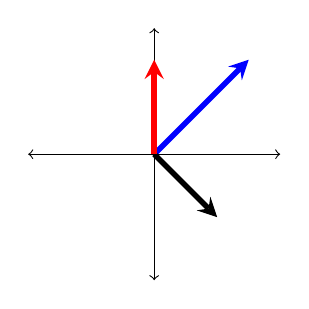
\begin{tikzpicture}[scale=0.8]
  \draw[<->] (-2,0)--(2,0);
  \draw[<->] (0,-2)--(0,2);
  
  \draw[line width=2pt,blue,-stealth](0,0)--(1.5,1.5);
  \draw[line width=2pt,-stealth](0,0)--(1,-1);
  \draw[line width=2pt,red,-stealth](0,0)--(0,1.5);

 \end{tikzpicture}
\end{image}
\end{problem}

\begin{problem}
\begin{multipleChoice}
 \choice[correct]{The vectors are linearly independent}
  \choice{The vectors are linearly dependent }
  \choice{There is not enough information given to make a determination }
 \end{multipleChoice}
\begin{image}[2in]
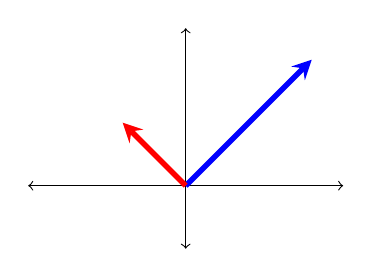
\begin{tikzpicture}[scale=0.8]
  \draw[<->] (-2.5,0)--(2.5,0);
  \draw[<->] (0,-1)--(0,2.5);
  
  \draw[line width=2pt,blue,-stealth](0,0)--(2,2);
  \draw[line width=2pt,red,-stealth](0,0)--(-1,1);

 \end{tikzpicture}
\end{image}
\end{problem}


\begin{problem}
\begin{multipleChoice}
 \choice[correct]{The vectors are linearly independent}
  \choice{The vectors are linearly dependent }
  \choice{There is not enough information given to make a determination }
 \end{multipleChoice}
\begin{image}
\tdplotsetmaincoords{70}{130}
\begin{tikzpicture}
	\draw[->](-2,0,0)--(2,0,0) node[below left]{$y$};
    \draw[->](0,-2,0)--(0,2,0) node[below left]{$z$};
    \draw[->](0,0,-2)--(0,0,2) node[below left]{$x$};
    \draw[->, line width=2pt,blue, -stealth](0,0,0)--(0,0,1);
    \draw[->, line width=2pt,red, -stealth](0,0,0)--(1,0,0);
    \draw[->, line width=2pt,orange, -stealth](0,0,0)--(0,1,0);
    
\end{tikzpicture}
\end{image}
\end{problem}

\end{problem}
\end{document} 